\section{Einleitung} % (fold)
\label{sec:einleitung}

Myonen gehören wie Elektronen zur Familie Leptonen und entstehen durch Pionen-Zerfall in den oberen Schichten der Atmosphäre.
In diesem Versuch wird die Lebensdauer dieser Myonen untersucht.

\section{Theorie} % (fold)
\label{sec:theorie}
\FloatBarrier
\subsection{Eigenschaften von Myonen} % (fold)
\label{sub:eigenschaften_von_myonen}

Myonen sind 206,77 mal schwerer als ein Elektronen und gehören zur zweiten Generation der Leptonenfamilie.
Zudem unterliegen diese nur der Schwachen und Elektromagnetischen Wechselwirkung und besitzen im gegensatz zu Elektronen eine endliche Lebensdauer.
\FloatBarrier
\subsection{Definition der Lebensdauer} % (fold)
\label{sub:definition_der_lebensdauer}

Der Zerfall von instabilen Teilchen ist ein statistischer Prozess, weshalb jedes Teilchen eine indivduelle Lebensdauer besitzt.
Eine allgemeine Definition der Lebensdauer ist über 

\begin{equation}
	\text{d}W = \lambda \text{d}t
\end{equation}

gegeben.

Bei dieser Definition ist die Wahrscheinlichkeit nicht explizit von $t$ abhängig, weshalb das Alter des Teilchens keine Rolle spielt.
Für $N$ zerfallende Teilchen ergiebt sich somit 

\begin{equation}
	\text{d}N = -N \text{d}W = -\lambda \text{d}t.
\end{equation}

Für große $N$ ergiebt sich näherungsweise für das Integral

\begin{equation}
	\frac{N(t)}{N_\text{0}} = \exp{(-\lambda t)},
\end{equation}

und somit für die Verteilung
 
\begin{equation}
	\frac{\text{d}N(t)}{N_\text{0}} = \lambda \exp{(-\lambda t)} \text{d}t .
\end{equation}
\\
Die charakteristische Lebensdauer $\tau$ wird über die Mittelwerte aller möglichen Lebensdauern gebildet, wobei diese mit der Häufigkeit ihres Vorkommens gewichtet sind.
Dies entspricht dem Ersten Moment der Verteilungsfunktion und es ergibt sich damit

\begin{equation}
	\tau = \int_\text{0}^\infty \lambda \exp{(-\lambda t)} \text{d}t = \frac{1}{\lambda} .
\end{equation}
\FloatBarrier
\subsection{Abschätzung der Lebensdauer mit Hilfe einer Stichprobe} % (fold)
\label{sub:abschaetzung_der_lebensdauer_mit_hilfe_einer_stichprobe}

Im Experiment lässt sich aus einer Stichprobe der Größe $n$ ein Wert für $\bar{t}$ über

\begin{equation}
	\bar{t} = \frac{1}{n} \sum_{\text{j=1}}^n t_\text{j}
\end{equation}

bestimmen.
Das Erste Moment von $\bar{t}$ ist die beste Näherung für $\tau$ und die beste Abschätzung des Fehlers ergibt sich aus

\begin{equation}
	s_{\bar{t}} = \frac{s}{\sqrt{n}}
\end{equation}

mit

\begin{equation}
	s^2 = \frac{1}{n-1} \sum_\text{j=1}^n \left(\bar{t} - t_\text{j}\right)^2 .
\end{equation}


Das Erste Moment von $s^2$ ist hierbei die Varianz $\sigma^2$ der nicht bekannten Verteilungsfunktion des Messproblems.
\FloatBarrier
\subsection{Bestimmung einer empirischen Verteilungsfunktion} % (fold)
\label{sub:bestimmung_einer_empirischen_verteilungsfunktion}


Beim Messen von Stichproben kann es durch Ausschließung sehr kleiner oder sehr großer Werte zu systematischen Fehlern kommen.
Eine andere Methode ist eine Abschätzung einer empirischen Verteilungsfunktion.
Dazu wird mit der \textit{Methode der kleinsten Quadrate} die Variablen $N_\text{0}$ und $\lambda$ variiert bis

\begin{equation}
	\sum_\text{j=1}^n \left(N(t_\text{j})-N_\text{0}\exp{(-\lambda t)}\right)^2 \stackrel{!}{=} \textbf{min}
\end{equation}

gilt, wobei $N(t_\text{j})$ die Häufigkeit des Messerbenisses $t_\text{j}$ darstellt.

Da die Nullsetzung der Ableitung zu transzendenten Gleichungen führt, wird das Gleichungssystem linearisiert und es ergibst sich für die Variablen

\begin{eqnarray}
	\lambda = \lambda_\text{A} + \alpha ,\\
	N_\text{0} = N_{\text{0}_\text{A}} + \beta.
\end{eqnarray}

Die Näherungswerte $\lambda_\text{A}$ und $N_{\text{0}_\text{A}}$ lasen sich Beispielsweise einer graphischen Darstellung von $\ln{N(t_\text{j})}$ gegen $t_\text{j}$ entnehmen, während die Korrekturterme $\alpha$ und $\beta$ durch geeignete Näherungen bestimmt werden können.
\FloatBarrier
\subsection{Bestimmung der Lebensdauer kosmischer Myonen} % (fold)
\label{sub:bestimmung_der_lebensdauer_kosmischer_myonen}

Kosmische Myonen können über einen Szintillationsdetektor nachgewiesen werden.
Die Myonen geben im Detektor kinetische Energie an die Szintillatormoleküle ab, welche dadurch angeregt werden.
Bei der Rückkehr in den Grundzustand werden Photonen im sichtbaren und nahen UV Bereich emittiert und der Lichtblitz kann über einen Sekundärelektronenvervielfacher (SEV) nachgewiesen werden.
Zerfällt das Myonen nun innerhalb des Detektors, kommt es zu einem weiteren Lichtblitz.
Aus der zeitlichen Differenz der beiden Lichtblitze kann nun die Lebensdauer bestimmt werden.
\FloatBarrier
\subsection{Eine Apparatur zur Lebensdauermessung} % (fold)
\label{sub:eine_apparatur_zur_lebensdauermessung}

\begin{figure}
	\centering
	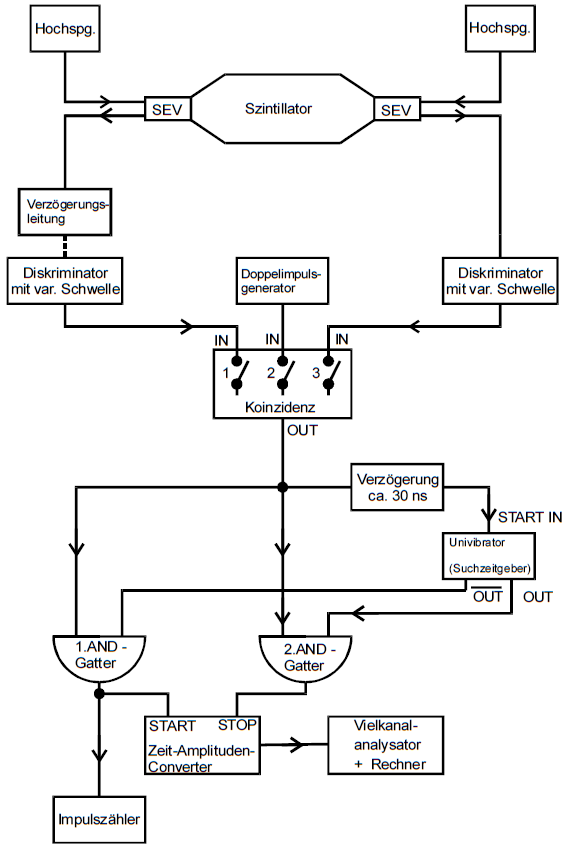
\includegraphics[width = 0.5\textwidth]{pic/schaltung.png}
	\caption{Blockschaltbild der Messapparatur \cite{anleitung}.}
	\label{schaltung}
\end{figure}

In Abbildung \ref{schaltung} ist das Blcokschaltbild der verwendeten Apparatur dargestellt.
Der Szintillationsdetektor hat ein Volumen von ca. $\SI{50}{\liter}$ und an den Stirnseiten ist je ein SEV angeschlossen.
Die zeitliche Differenz der Lichtimpluse kann mithilfe eines Zeit-Amplituden-Konverters (TAC) über die \textit{Stopuhr-Methode} gemessen werden.
Der Impuls des einfallenden Myons startet dabei die Zeitmessung, während der Impuls des zerfallenden Myons diese beendet.
Dies ist möglich, da die Abklingdauer der Lichtpuls mit $\SI{10}{\nano\meter}$ im Detektor klein gegen die Lebensdauer ist.
Der TAC erzeugt einen Spannungsimpuls proportional zum Zeitdifferenz und leitet diesen an einen Vielkanalanalysator weiter.\\

Nicht alle Myonen die einen Startimpuls erzeugen führen auch zu einem Stopimpuls.
Daher ist es nötig nach einer Suchzeit $T_\text{S}$ abzubrechen.
Diese sollte ein Vielfaches der Lebensdauer betragen, aber klein gegen den mittleren Abstand zweier Startimpulse sein.
Um dies zu realisierenm, wird eine monostabile Kippstufe verwendet. 
Diese leitet nur einen Impuls an den Stop-Eingang des TAC weiter, wenn in der Zeit $T_\text{S}$ ein weiterer Imulps auftritt, ansonsten kehrt sie wieder in den Ausgangszustand zurück.

Es kann jedoch passieren, dass zwei Myonen innerhalb der Zeit $T_\text{S}$ den Detektor durchlaufen.
Diese tragen dann zur statistisch verteilten Untergrundrate $U$ bei, welche sich berechnen und somit herausrechnen lässt. \\

Weiterhin kann es zur Auslösung eines Signals durch thermische Elektronen kommen.
Da die Signale meist klein sind im Vergleich zu den Lichtsignalen der Myonen können sie mithilfe einer Diskriminator Schweller herausgefiltert werden.
Um zudem größere Signale herauszufiltern sind an jeder Seite des Detektors SEV angebracht.
Die von diesen erzeugten Signale werden an eine Koinzidenzschaltung weitergegeben.
Der eintreffende Impuls wird nur weitergegeben, wenn von beiden SEV in einem kleinen Zeitabstand von ca. $\SI{4}{\nano\second}$ ein Signal eintrifft.
Um die Laufzeit- und Verstärkungsunterschiede der beiden SEV anzugleichen, wird eine Verzögerungsleitung und eine geeignete Wahl der Diskriminatorschwelle verwendet.
\FloatBarrier
\section{Messprogramm} % (fold)
\label{sec:messprogramm}

\begin{enumerate}
	\item Bestimmung der Lebensdauern des Myons aus einer Messreihe von Individuallebensdauern mit einer Messzeit von drei Tagen.
\end{enumerate}